% EvoCrypt manuscript adapted from sn-article.tex to the Springer LNCS class.
% Compile from this directory with pdflatex, bibtex, pdflatex, pdflatex.
\documentclass[runningheads]{llncs}

\usepackage[T1]{fontenc}
\IfFileExists{newtxtext.sty}{%
  \usepackage{newtxtext}%
  \IfFileExists{newtxmath.sty}{\usepackage[varvw]{newtxmath}}{}%
}{}
\usepackage{graphicx}
\usepackage{multirow}
\usepackage{amsmath,amssymb,amsfonts}
\usepackage{mathrsfs}
\usepackage{xcolor}
\usepackage{textcomp}
\usepackage{booktabs}
\usepackage{tabularx}
\usepackage{algorithm}
\usepackage{algorithmicx}
\usepackage{algpseudocode}
\usepackage{listings}

\begin{document}

\title{EvoCrypt: An Upgradable Cryptographic Coprocessor for the Ethereum Virtual Machine}
\titlerunning{EvoCrypt: An Upgradable Cryptographic Coprocessor}

\author{Qi Liu\inst{1} \and
Qianhong Wu\inst{1} \and
Bo Qin\inst{2}}
\authorrunning{Q. Liu et al.}

\institute{School of Cyber Science and Technology, Beihang University, Beijing 100191, China
\and School of Information, Renmin University of China, Beijing 100872, China}

\maketitle

\begin{abstract}
Smart contracts frequently rely on cryptographic algorithms, yet implementing complex cryptographic computation in Solidity expands it into large sequences of EVM instructions, resulting in substantial execution overhead and gas consumption. Precompiled contracts reduce these costs by exposing client-native routines at fixed addresses, but they provide no runtime mechanism for evolving an algorithm independently of client releases and coordinated network upgrades. We present EvoCrypt, an upgradeable cryptographic coprocessor that exposes a stable contract-facing interface while executing replaceable WebAssembly modules in a controlled client-side runtime. EvoCrypt distributes version metadata on-chain and deterministically activates an installed module at a designated block height, allowing participating nodes to switch algorithm versions consistently. Each invocation is charged according to a deterministic algorithm-level gas schedule associated with the activated version, thereby avoiding the cost of expanding the algorithm into EVM instructions while retaining explicit resource accounting. We implement EvoCrypt in Geth and evaluate it on a 20 node private Clique network configured with zero-period block production to isolate system-level upgrade overhead from the block interval. Measured \emph{network-wide upgrade duration} is the Geth-side time to finish upgrade handling on all evaluated nodes---from RPC submission through receipt observation, event handling, and node-local WASM preparation---and excludes network propagation and consensus delay; under this definition the prototype completes upgrades within 0.54--2.34~ms across the eight evaluated algorithms. EvoCrypt achieves execution latency comparable to Solidity implementations on lightweight algorithms, with up to 48\% lower latency on computation-heavy workloads.

\keywords{blockchain \and smart contracts \and upgrade \and WebAssembly}
\end{abstract}

\section{Introduction}\label{sec1}

Blockchain systems are increasingly used in digital finance, supply-chain management, digital identity, and trusted data exchange, and have evolved from narrowly scoped distributed ledgers into programmable trusted computing platforms \cite{nakamoto2008bitcoin,zou2021smartContracts}. Smart contracts provide the core mechanism for this programmability: they execute predefined rules for asset transfer, authorization, state update, and multi-party coordination within a deterministic blockchain execution environment \cite{woodEthereumYellowPaper,ethereumEVM}. These operations commonly depend on cryptographic functions for identity authentication, data integrity, digital signatures, and privacy protection, so smart contracts require ways to invoke or execute cryptographic algorithms to support trustworthy on-chain business logic. At the same time, advances in quantum computing challenge the long-term security assumptions of deployed public-key cryptography \cite{shor1999,grover1996}, and the standardization of post-quantum cryptographic algorithms has made post-quantum migration an important requirement for long-term blockchain security \cite{nistPqcProject}. Because many on-chain workflows expose cryptographic capabilities through smart contracts, this migration requires not only support for new cryptographic algorithms in the underlying blockchain client but also timely access to these capabilities from smart contracts. Providing extensible and evolvable support for contract-facing cryptographic algorithms has therefore become an important problem for blockchain systems designed for long-term security evolution.

Ethereum currently offers two common routes for executing cryptographic logic. A developer can implement an algorithm directly in Solidity, which keeps the logic flexible and deployable at the contract layer but executes the computation through Ethereum Virtual Machine (EVM) instructions \cite{woodEthereumYellowPaper,ethereumEVM}. That path imposes two recurring obstacles for contract-facing cryptography. The first is an engineering obstacle: complex arithmetic, byte-oriented workloads, and correctness-sensitive logic must be expressed as EVM bytecode, which makes non-trivial cryptographic implementations difficult to develop, audit, and maintain. The second is an economic obstacle: gas prices computation at instruction level \cite{woodEthereumYellowPaper,buterin2016eip150}, so a cryptographic algorithm expanded into a long EVM instruction sequence is charged for every opcode it executes. We refer to this effect as \emph{gas amplification}: the gas of an in-contract implementation grows with its expanded instruction count rather than with the algorithmic work performed, and computationally intensive Solidity implementations therefore incur substantial execution latency and gas overhead. Alternatively, Ethereum clients can expose selected algorithms as Precompiled Contracts, which execute native client code behind predefined EVM interfaces \cite{evmCodesPrecompiled}. This route lowers execution cost for algorithms already fixed in the protocol catalog, but it does not provide a general contract-layer way to add arbitrary new cryptographic workloads without a client release, and it binds each exposed routine to the client software. Updating a Precompiled Contract normally requires modifying client source code, rebuilding the client, and coordinating deployment across nodes.

This split leaves a capability gap relative to those Solidity obstacles. When a required algorithm is not available as a precompile, in-contract Solidity remains the default deployment path, yet it remains poorly matched to expensive cryptographic computation. Precompiled Contracts improve execution efficiency for a fixed set of routines but are difficult to update independently of the client release process and do not by themselves address algorithm evolution requirements such as post-quantum migration. More generally, smart contract engineering already faces persistent challenges around correctness, cost, and maintainability \cite{zou2021smartContracts}. Prior work has examined live-upgradable blockchain clients and automated smart-contract patching \cite{wang2023phoenix,rodler2021evmpatch}, showing the broader relevance of upgradeability in blockchain software. For cryptographic algorithms, however, the challenge is to support algorithm replacement without changing the semantics of historical execution or allowing different nodes to select different algorithm versions at the same block height. A process-local plugin or shared-library boundary ties execution to platform-specific native binaries and weakens the goal that every node apply the same algorithm semantics at the same block. Existing approaches do not directly provide a low-intrusion mechanism for replacing contract-facing cryptographic implementations with a uniform, portable module payload while preserving deterministic activation across nodes.

This paper proposes a general Cryptographic Coprocessor architecture for smart-contract-enabled blockchain clients. The coprocessor decouples the contract-facing cryptographic algorithm interface from the WASM module implementation managed by the client. Smart contracts invoke a stable EVM-facing interface to obtain cryptographic results without embedding the algorithm in contract bytecode, while the client maintains replaceable WASM algorithm modules behind that interface. The upgrade path combines on-chain coordination with off-chain asynchronous preparation: an upgrade transaction records metadata and emits an event, while client-side listeners verify, compile, and instantiate the target WASM module outside the EVM execution critical path of that transaction. To prevent nodes from switching versions according to local readiness time, the protocol separates asynchronous upgrade preparation from deterministic activation through an Activation Block. Because algorithm execution is moved behind the coprocessor boundary, the invocation path charges a deterministic algorithm-level gas schedule registered in the on-chain version metadata instead of metering an expanded EVM instruction sequence, so contract-facing cryptographic calls are not subject to gas amplification.

The main contributions of this article are summarized as follows.
\begin{itemize}
    \item Firstly, we design a Cryptographic Coprocessor that separates contract-facing cryptographic algorithm interfaces from WASM module implementations, allowing algorithm implementations to be managed and replaced independently of the core EVM execution logic while using a narrower runtime boundary than process-local plugin loading.
    \item Secondly, we design an upgrade protocol that combines on-chain event coordination, off-chain asynchronous WASM preparation, and block-height-based deterministic activation.
    \item Finally, we implement a prototype of EvoCrypt and evaluate it on a 20-node private blockchain network. Experimental results show that algorithm-level gas pricing decouples per-invocation cost from the expanded EVM instruction count, thereby avoiding the opcode-level gas amplification observed in Solidity executions; the registered prices in the evaluated prototype are experimental parameters, so the results demonstrate the pricing mechanism and the resulting capability extension rather than a calibrated magnitude of gas savings.
\end{itemize}
The resulting claims are intentionally bounded: the evaluation concerns contract-facing cryptographic algorithms under the evaluated scenarios, does not claim that unrelated EVM transactions are unaffected during the upgrade preparation window, does not set up a separate consistency experiment, and does not treat the WASM sandbox as a formal security proof.

\section{Related Work}\label{sec2}


Existing blockchain upgrade schemes primarily replace code at the protocol or client level, where a coordinated version transition preserves a common execution rule across nodes. Cardano's hard-fork combinator moves the chain between protocol eras at designated upgrade points, while work on updatable blockchains studies synchronization between old and new chains \cite{cardanoHardForkCombinator,cardanoEvolution,ciampi2020updatable}. Soft-fork approaches instead place selected policy changes within rules that can be adopted without replacing the entire protocol \cite{zindros2021softPower}. Phoenix extends this direction by embedding upgrade code in blockchain transactions and compiling it at runtime. Polkadot stores WASM-based runtime logic on chain and activates governance-approved replacements during block synchronization \cite{wang2023phoenix,polkadotRuntimeUpgrades}. These approaches support chain-wide or client-wide evolution, but they require protocol coordination and place the replacement boundary across a substantial portion of system execution.

Contract-level schemes update application logic without replacing the entire blockchain client, using deployable contracts, proxy indirection, or bytecode rewriting. EVMPatch automatically patches deployed Ethereum smart contracts through bytecode rewriting and proxy-based deployment, while Solidity implementations offer application-level flexibility within the EVM \cite{rodler2021evmpatch,ethereumEVM}. LEAGAN further extends contract-level upgradeability through data separation, incremental hashing, revision control, and status-contract-based version management, enabling contract logic to evolve while preserving persistent state and supporting non-halt deployment \cite{kumar2025leagan}.Precompiled Contracts provide a complementary client-native path for selected cryptographic routines through reserved EVM-facing addresses \cite{evmCodesPrecompiled,eip196,eip197}. These mechanisms avoid some forms of client redeployment. Contract-level implementations remain constrained by EVM execution cost and state or interface compatibility, whereas adding or replacing a Precompiled Contract normally requires changes to client and protocol rules.



Dynamic software-update schemes move replacement below the application layer by loading new components into a running host, with emphasis on availability, version compatibility, or isolation. KylinX supports runtime library replacement through dynamic mapping, Mvedsua combines dynamic updates with multi-version execution, PYLIVE changes Python code online, and distributed-system research addresses modular updates and version consistency \cite{zhang2018kylinx,pina2019mvedsua,huang2021pylive,ajmani2006modular,baresi2017versionConsistency}. WASM provides a portable artifact format and explicit host boundary for this style of replacement. In blockchain systems, existing WASM-based upgrades generally target broad runtime logic rather than a narrow EVM-facing cryptographic interface \cite{webassemblyCoreSpec,polkadotRuntimeUpgrades}. The Cryptographic Coprocessor addresses this narrower boundary by keeping the EVM-facing call interface stable, preparing replaceable WASM modules asynchronously, and selecting versions through chain-derived metadata and an Activation Block.


\section{EvoCrypt Design}\label{sec3}

The Cryptographic Coprocessor provides runtime-upgradable WASM implementations for contract-facing cryptographic algorithms without turning the entire blockchain client into a dynamically updated component. We specify the design by three objects reused by the protocols below: a version metadata record $\mu_{a,v}$, a height-based version selector $v^{*}(a,b)$, and an algorithm-level gas schedule $G(a,v,x)$. Algorithm logic is shipped as portable WASM bytecode rather than per-node native binaries, so heterogeneous clients execute the same module artifact under the same selection rule. Ordinary transactions continue through the EVM under unchanged opcode-level pricing. Only selected cryptographic implementations behind a stable contract-facing interface are prepared, loaded, and selected as replaceable WASM modules.

\subsection{Overview}\label{sec3.1}
Figure~\ref{fig:overview} shows the main modules. The Execution Engine executes ordinary EVM transactions. Identity Hooks recognize calls to the Management Contract entry point used by the prototype and route only those calls into the coprocessor boundary. The Cryptographic Coprocessor manages ABI decoding, algorithm lookup, version selection, gas metadata, and WASM invocation. The Upgrade Handler listens for on-chain upgrade events and prepares node-local artifacts. The WASM Runtime compiles and instantiates modules under a controlled import/export and memory boundary, and WASM Modules contain the replaceable algorithm implementations.

\begin{figure}[!tb]
\centering
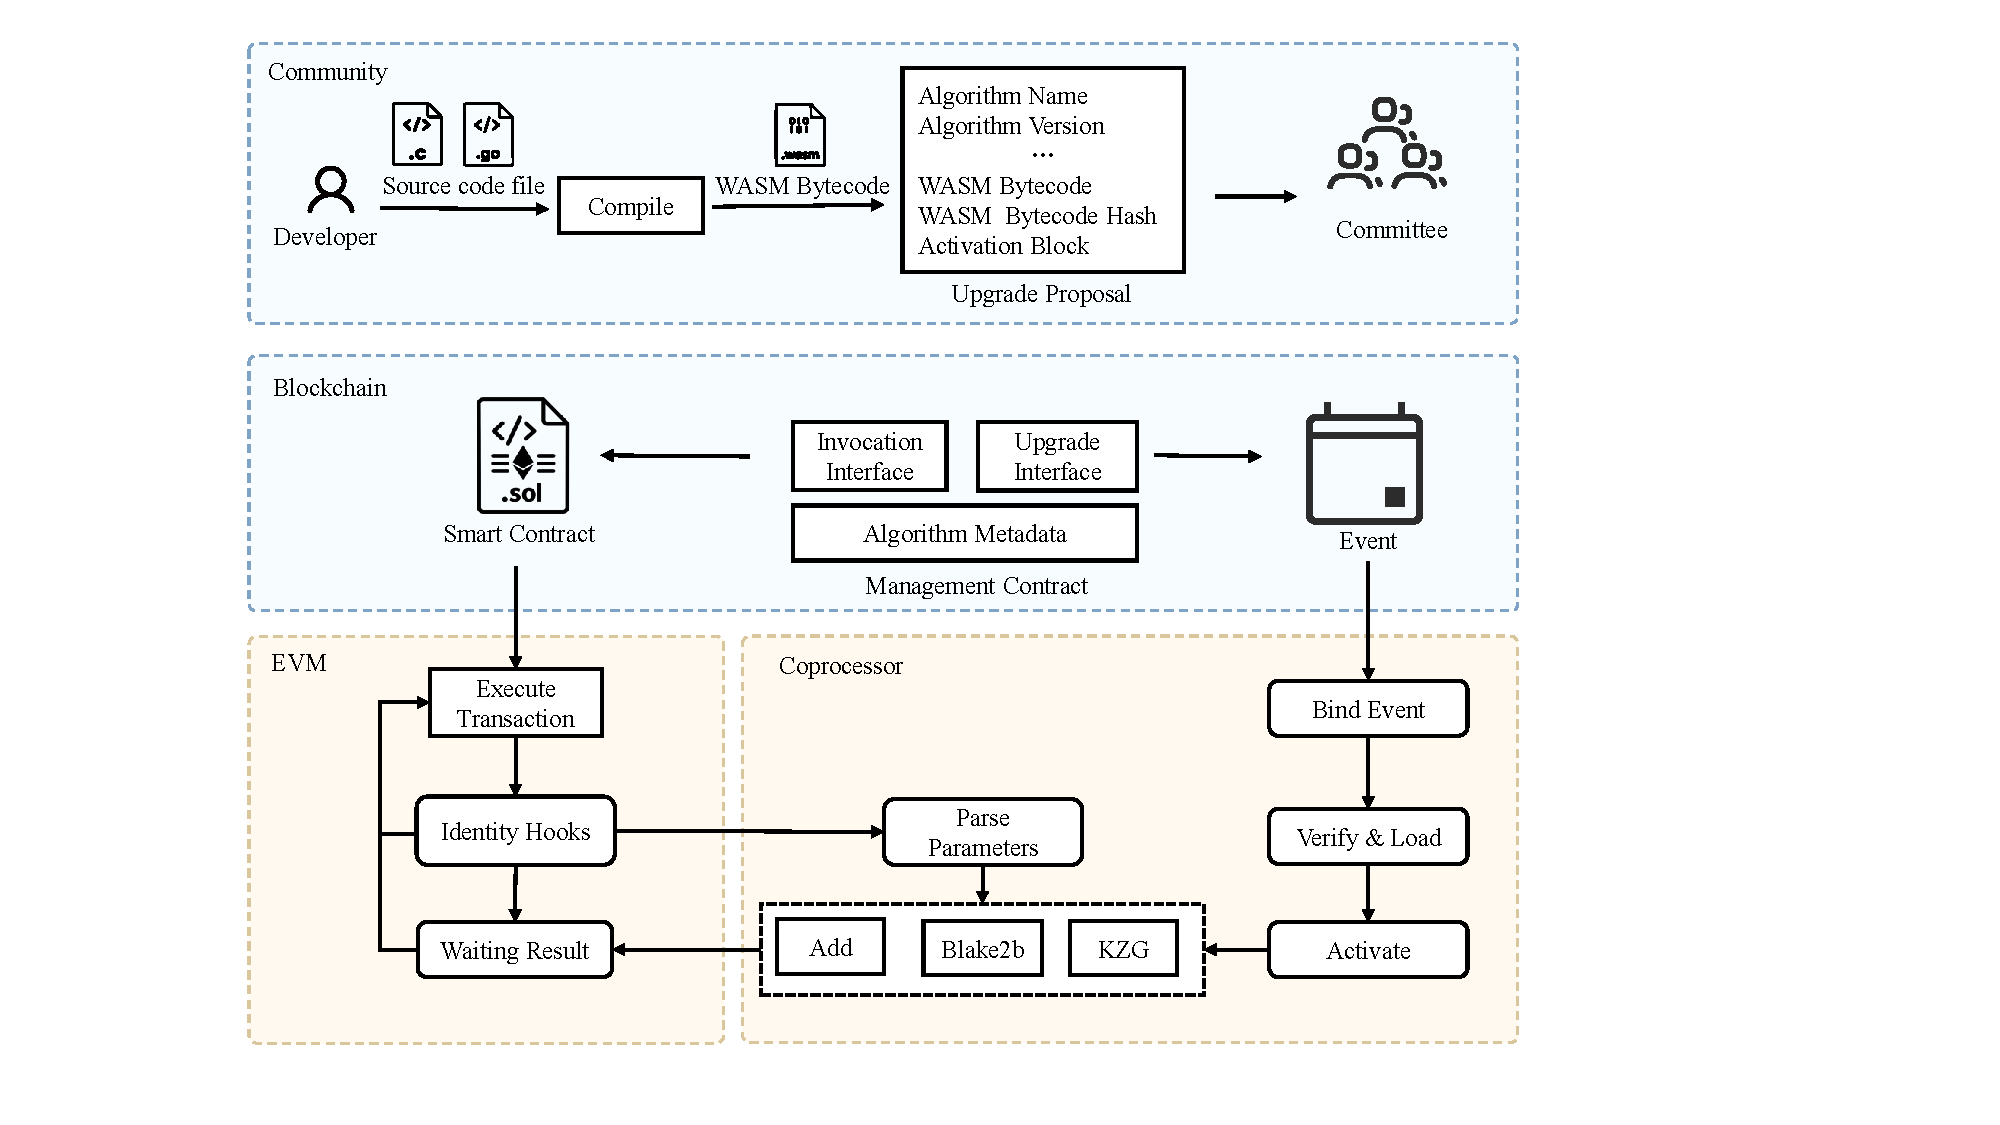
\includegraphics[width=\textwidth]{../image/overview.pdf}
\caption{Workflow of the Upgradable Cryptographic Coprocessor.}
\label{fig:overview}
\end{figure}

The on-chain layer contains the Management Contract, event log, version metadata, and Activation Block. The Management Contract abstracts the CodeStorage contract used in the prototype: its invocation interface exposes the contract-facing call entry, and its upgrade interface publishes the metadata record defined in~\eqref{eq:version-metadata}. Clients derive the module hash from the decoded artifact during local preparation. The client-side layer contains the Execution Engine, Identity Hooks, Cryptographic Coprocessor, Upgrade Handler, WASM Runtime, and local module workspace. This split keeps the chain as the authoritative coordination surface while leaving module preparation as node-local work. Section~\ref{sec3.2} defines the metadata record and the upgrade protocol that publishes it. Section~\ref{sec3.3} defines the invocation path and the gas schedule that charges a call to the selected version.

\subsection{Upgrade Protocol}\label{sec3.2}
An upgrade starts from an on-chain proposal. In the versioned path, a committee-authorized proposer submits the proposal through \texttt{uploadCodeVersion}, and the Management Contract admits it only after the committee reaches consensus on its contents. During transaction execution, the contract stores the admitted record and emits a versioned upgrade event. The EVM path does not compile or instantiate the WASM module; it records the authoritative metadata and publishes an event that clients can observe.

\begin{definition}[Version metadata]
\label{def:version-metadata}
Let $a$ be an algorithm name and $v$ a version number. An admitted upgrade is the metadata record
\begin{equation}
\mu_{a,v}=\bigl(a,\,v,\,C_{a,v},\,h_{a,v},\,g^{(0)}_{a,v},\,\lambda_{a,v},\,\tau^{\mathrm{in}}_{a,v},\,\tau^{\mathrm{out}}_{a,v},\,H_{a,v}\bigr),
\label{eq:version-metadata}
\end{equation}
where $C_{a,v}$ is the compiled WASM bytecode, $h_{a,v}=\mathrm{Keccak256}(C_{a,v})$ is the module hash, $g^{(0)}_{a,v}$ is the initial gas fee, $\lambda_{a,v}$ is the gas slope parameter, $\tau^{\mathrm{in}}_{a,v}$ and $\tau^{\mathrm{out}}_{a,v}$ are the ABI input and output type descriptors, and $H_{a,v}$ is the Activation Block height. The Management Contract stores an encoding of these fields. Each node recomputes $h_{a,v}$ from the decoded bytecode during preparation and binds that hash to the prepared version.
\end{definition}

Table~\ref{tab:version-metadata} summarizes the components of $\mu_{a,v}$. Write $\mathcal{V}_{a}$ for the set of versions already registered for algorithm $a$. The chain is the sole source of $\mu_{a,v}$; the upgrade event carries only $\langle a,v,H_{a,v}\rangle$ as a notification index.

\begin{table}[ht]
\centering
\caption{Components of the version metadata record $\mu_{a,v}$.}\label{tab:version-metadata}
\begin{tabular}{llp{0.55\textwidth}}
\toprule
Symbol & Field & Role \\
\midrule
$a$ & algorithm name & Identifier of the contract-facing algorithm. \\
$v$ & algorithm version & Monotone version number within $\mathcal{V}_{a}$. \\
$C_{a,v}$ & WASM bytecode & Compiled module artifact executed by the runtime. \\
$h_{a,v}$ & module hash & Keccak-256 digest of $C_{a,v}$, bound at preparation. \\
$g^{(0)}_{a,v}$ & initial gas fee & Constant term of the invocation schedule~\eqref{eq:gas-price}. \\
$\lambda_{a,v}$ & gas slope parameter & Per-byte coefficient of the invocation schedule. \\
$\tau^{\mathrm{in}}_{a,v}$ & input type & ABI descriptor of the call-stage inner input. \\
$\tau^{\mathrm{out}}_{a,v}$ & output type & ABI descriptor of the returned result. \\
$H_{a,v}$ & activation height & First block at which version $v$ may become active. \\
\bottomrule
\end{tabular}
\end{table}

Each client runs an Event Listener for Management Contract upgrade events. When a listener observes $\langle a,v,H\rangle$, it recovers $\mu_{a,v}$ through \texttt{getVersionInfo}, checks that the event and stored record agree on $v$ and $H_{a,v}$, and delegates preparation to the Upgrade Handler. The handler decodes $C_{a,v}$, computes $h_{a,v}$, asks the WASM Runtime to compile and instantiate the module, validates the required \texttt{execute} export, and records $(a,v)$ as a prepared version.

This workflow separates on-chain coordination from node-local preparation. The chain provides one admitted record $\mu_{a,v}$, while each node independently verifies and prepares the same artifact. Under the mandatory-upgrade policy, a node that observes a valid upgrade event must complete preparation of $(a,v)$ before treating that version as callable. A failed attempt retries from the contract record and does not roll back the already executed upgrade transaction. The upgrade transaction therefore does not wait for WASM compilation. Algorithm~\ref{alg:upgrade-protocol} summarizes the protocol.

\begin{algorithm}[!tb]
\caption{\textbf{Activation-Block-based WASM upgrade protocol.}}
\label{alg:upgrade-protocol}
\begin{algorithmic}[1]
\Require Metadata $\mu_{a,v}$ as in~\eqref{eq:version-metadata}; node set $\mathcal{N}$
\Ensure Prepared set updated on every $n_i\in\mathcal{N}$
\State committee-authorized proposer submits \texttt{uploadCodeVersion}$(\mu_{a,v})$
\State Management Contract stores $\mu_{a,v}$; emits event $\langle a,v,H_{a,v}\rangle$
\ForAll{$n_i\in\mathcal{N}$}
    \State observe $\langle a,v,H_{a,v}\rangle$; fetch $\mu'_{a,v}$ from Management Contract
    \If{event fields disagree with $\mu'_{a,v}$}
        \State reject $(a,v)$
    \Else
        \State decode $C_{a,v}$; set $h_{a,v}\gets\mathrm{Keccak256}(C_{a,v})$
        \Repeat
            \State compile and instantiate; validate \texttt{execute} export
        \Until{preparation succeeds}
        \State persist $h_{a,v}$ and $\mu_{a,v}$; mark $(a,v)$ prepared
    \EndIf
\EndFor
\end{algorithmic}
\end{algorithm}

Asynchronous preparation would break execution consistency if nodes switched versions as soon as local compilation finished. Two nodes may observe the same chain but complete preparation at different wall-clock times. The coprocessor therefore separates preparation from activation through $H_{a,v}$. Figure~\ref{fig:upgrade-protocol} shows this two-phase timeline on the blockchain node network.

\begin{figure}[!tb]
\centering
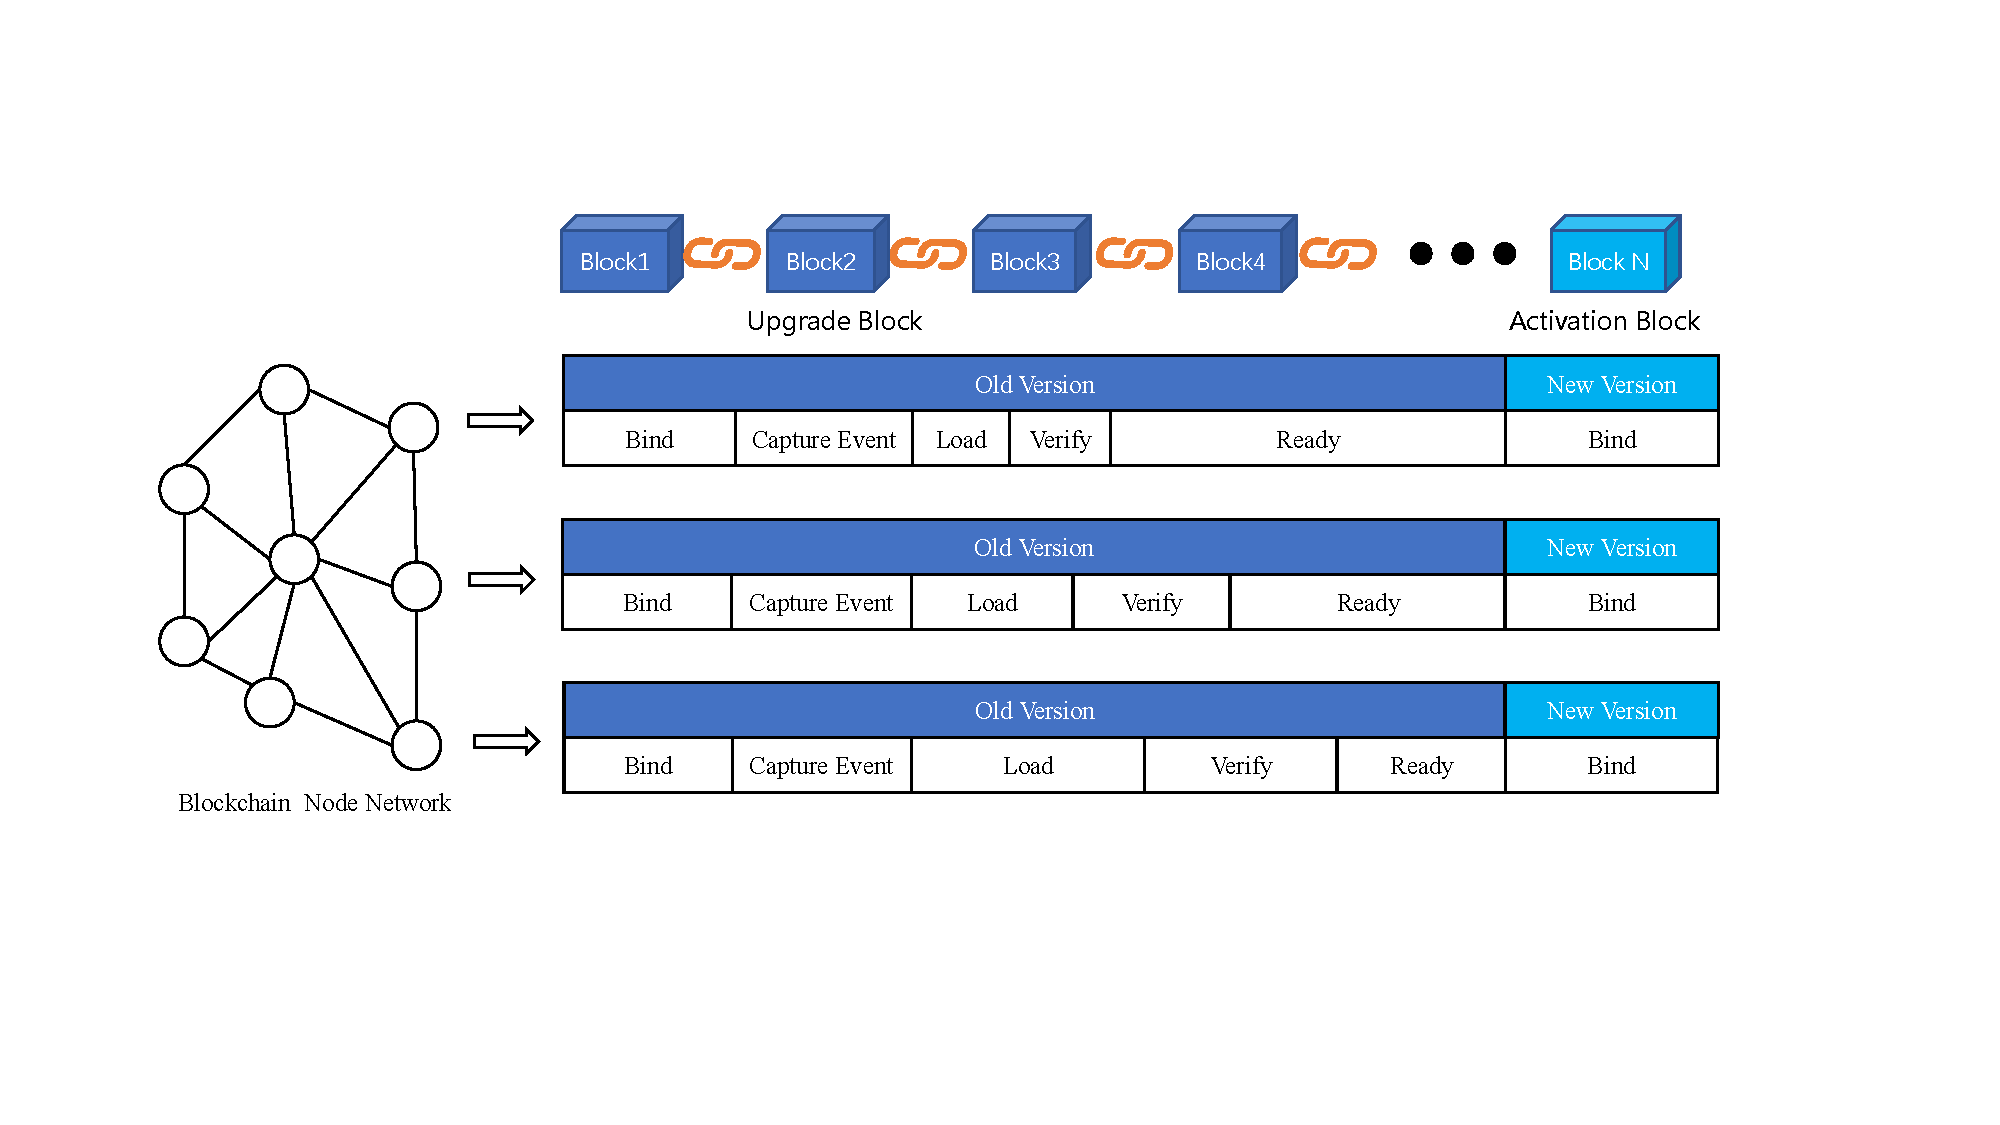
\includegraphics[width=\textwidth]{../image/upgrade_protocol.pdf}
\caption{Node-local preparation and deterministic network-wide activation of an EvoCrypt upgrade.}
\label{fig:upgrade-protocol}
\end{figure}

The Upgrade Block is the block that includes the admitted \texttt{uploadCodeVersion} transaction and emits $\langle a,v,H_{a,v}\rangle$. After that inclusion, each node independently captures the event, recovers $\mu_{a,v}$, and completes the off-chain Load--Verify--Ready sequence of Algorithm~\ref{alg:upgrade-protocol}. Invocations in this interval still use the previously selected version: local readiness does not change which implementation is served. When the chain reaches the Activation Block $H_{a,v}$, nodes that share the same chain view bind version $v$ together. The next definition makes this height-based switch precise.

\begin{definition}[Active version]
\label{def:active-version}
Let $\mathcal{V}_{a}$ be the registered version set of algorithm $a$, and let $b$ be the execution block height. The version used at height $b$ is
\begin{equation}
v^{*}(a,b)=
\underset{v \in \mathcal{V}_{a}}{\arg\max}
\left\{
\left(H_{a,v},\,v\right)
\;\middle|\;
H_{a,v} \leq b
\right\}.
\label{eq:version-select}
\end{equation}
The $\arg\max$ is lexicographic on the pair $(H_{a,v},v)$: among versions whose activation height does not exceed $b$, the rule prefers the latest activation height and, for a tied height, the larger version number. If the feasible set is empty, no version is active and the invocation fails with a missing-version error.
\end{definition}

Equation~\eqref{eq:version-select} makes activation a function of chain height rather than local readiness. Given the same chain view and the same $\{\mu_{a,v}\}_{v\in\mathcal{V}_{a}}$, every node computes the same $v^{*}(a,b)$. The protocol is a forced upgrade: once $v^{*}(a,b)$ is defined, a node must execute that version and must not serve an obsolete implementation. If $(a,v^{*}(a,b))$ is not yet prepared when a call arrives or when height $b$ is processed, the node reloads $\mu_{a,v^{*}(a,b)}$ from the Management Contract and completes validation, compilation, and instantiation before proceeding.

\subsection{Invocation Protocol}\label{sec3.3}
The Invocation Protocol exposes a uniform contract-facing interface. A caller supplies the algorithm name $a$ and an ABI-encoded input $x$ that conforms to $\tau^{\mathrm{in}}_{a,v^{*}(a,b)}$. The contract does not depend on the artifact location, implementation language, or local loading state. It depends only on the EVM-facing boundary and on the ABI contract of the selected version. If $v^{*}(a,b)$ is not yet prepared, the coprocessor reloads $\mu_{a,v^{*}(a,b)}$ and completes compilation before execution, rather than redirecting the call to an obsolete implementation.

Inside the client, the EVM integration boundary recognizes the CodeStorage target and the \texttt{callFunc} selector, then parses the outer calldata and normalizes $a$. The inner input $x$ remains ABI-encoded across the host--runtime boundary: a dynamically upgraded WASM module receives these bytes through its \texttt{execute} export and returns an ABI-encoded result, whereas a built-in routine may decode and re-encode the values in the host. In both cases the selected result is returned to the EVM call frame. Replacing an implementation therefore does not change the contract-facing call shape, provided that $\tau^{\mathrm{in}}_{a,v}$ and $\tau^{\mathrm{out}}_{a,v}$ remain compatible.

At the data plane, a caller encodes the typed parameters with $\tau^{\mathrm{in}}_{a,v^{*}(a,b)}$, wraps them in a \texttt{callFunc(string,bytes)} envelope, and issues a read-only \texttt{STATICCALL} to CodeStorage. Calls whose selector is \texttt{callFunc} enter the invocation path; other CodeStorage selectors continue through metadata or management dispatch; all other addresses follow ordinary EVM routing. The dispatcher parses $(a,x)$, computes $v^{*}(a,b)$ by~\eqref{eq:version-select}, and blocks on forced preparation when the mandatory-upgrade policy applies. It then charges the deterministic fee defined below, executes the selected WASM module, and returns the ABI-encoded output. Invalid calldata, a missing version, insufficient gas, or a runtime failure surface as explicit errors. Algorithm~\ref{alg:invocation-protocol} summarizes this flow.

\begin{definition}[Algorithm-level gas schedule]
\label{def:gas-schedule}
Each algorithm version uses an independent pricing rule. A call with inner input $x$ against version $v$ of algorithm $a$ is charged
\begin{equation}
G(a,v,x)=g^{(0)}_{a,v}+\lambda_{a,v}\cdot |x|,
\label{eq:gas-price}
\end{equation}
where $|x|$ is the byte length of the call-stage inner input, $g^{(0)}_{a,v}$ is the initial gas fee, and $\lambda_{a,v}$ is the gas slope parameter registered in $\mu_{a,v}$. The charged amount does not depend on node-local CPU time or on the number of WASM instructions executed inside the module.
\end{definition}

\begin{algorithm}[!tb]
\caption{\textbf{Contract-to-coprocessor invocation protocol.}}
\label{alg:invocation-protocol}
\begin{algorithmic}[1]
\Require Caller contract, algorithm name $a$, typed input $p$, block height $b$, gas budget $g$
\Ensure ABI-encoded result $y$ or explicit error
\State build \texttt{callFunc} calldata $d$ from $p$; issue \texttt{STATICCALL} to CodeStorage with gas $g$
\If{target is not CodeStorage \texttt{callFunc}}
    \State continue ordinary EVM or management dispatch; \textbf{return}
\EndIf
\If{calldata parsing fails}
    \State \textbf{return} ABI error
\EndIf
\State parse $(a,x)$ from $d$; set $v\gets v^{*}(a,b)$ by~\eqref{eq:version-select}
\If{no applicable version $v$}
    \State \textbf{return} missing-version error
\EndIf
\If{$(a,v)$ not prepared}
    \Repeat
        \State forcibly reload $\mu_{a,v}$ and prepare $(a,v)$
    \Until{$(a,v)$ prepared}
\EndIf
\State $G_{\mathrm{req}}\gets G(a,v,x)$ by~\eqref{eq:gas-price}
\If{$g<G_{\mathrm{req}}$}
    \State \textbf{return} out-of-gas error
\EndIf
\State charge $G_{\mathrm{req}}$; $y\gets\mathrm{WASM}(a,v,x)$
\State \textbf{return} $y$, or runtime error on failure
\end{algorithmic}
\end{algorithm}

Equation~\eqref{eq:gas-price} is what removes opcode-level gas amplification from the invocation path. The fee is computed from the selected version's registered coefficients and from $|x|$, not from metering the module's internal execution, and it is identical for every node that resolves the same $v^{*}(a,b)$ on the same input. The pair $(g^{(0)}_{a,v},\lambda_{a,v})$ is therefore an explicit per-version policy: it can reflect the algorithm's resource class rather than the expanded instruction count of an equivalent EVM implementation. The algorithm-level schedule is charged only on the \texttt{callFunc} path. Upgrade and metadata transactions remain under ordinary transaction pricing. The coefficients used in Section~\ref{sec5} are experimental parameters; they demonstrate this charging mechanism rather than a calibrated economic optimum.

\section{Security Analysis}\label{sec4}

\subsection{Attack Circumstances}\label{sec4.1}
The security analysis focuses on attack circumstances introduced by cryptographic algorithms that are upgraded at runtime and invoked from contracts. Upgrade submission is restricted to committee-authorized proposers (Section~\ref{sec4.2}), so the analysis distinguishes two adversary positions. An external attacker may craft transaction inputs and exert timing pressure around node-local upgrade preparation but cannot register artifacts or metadata fields. A faulty or compromised admitted proposer may influence uploaded artifacts and metadata fields. We also consider erroneous upgrade artifacts and local preparation failures because they can lead to the same safety outcomes as adversarial inputs. The analysis does not model a compromised Geth binary, a broken consensus protocol, a captured committee, or cryptographic primitives whose mathematical assumptions are false.

\noindent\textbf{Malicious or malformed WASM artifacts.}
A faulty or compromised admitted proposer may submit a WASM module that is malformed, omits the required entry point, imports unauthorized host functions, declares unsafe memory behavior, or attempts to exploit the WASM runtime boundary. This scenario targets execution isolation: the module is dynamically supplied after client deployment, so the client cannot rely on source-level review or static compilation into the Geth binary.

\noindent\textbf{Inconsistent upgrade metadata.}
An attacker or faulty proposer may publish metadata whose version, Activation Block, gas parameters, ABI type descriptors, event projection, or encoded artifact are inconsistent with the intended upgrade. Such inconsistencies can cause version confusion, incorrect ABI decoding, incorrect gas charging, or preparation of an artifact that does not correspond to the version later selected during EVM execution.

\noindent\textbf{Resource-exhaustion attempts.}
Dynamic algorithm loading creates denial-of-service risks. A module may be large, slow to compile, memory intensive, or designed to run for a long time. A low gas setting may underprice an expensive cryptographic operation, and large uploaded artifacts may increase calldata, storage, propagation, and data-availability pressure.

\noindent\textbf{Asynchronous readiness divergence.}
Nodes may observe the same on-chain upgrade event but complete WASM validation, compilation, instantiation, and local persistence at different wall-clock times. A node may also fail to prepare the required artifact. If local readiness time or local wall-clock time were used for version selection, nodes executing the same block could resolve the same contract-facing call to different algorithm implementations.

\subsection{Security Solutions}\label{sec4.2}
The proposed coprocessor addresses these attack circumstances through committee-gated upgrade admission, sandboxed WASM execution, authoritative metadata recovery, deterministic resource accounting, and Activation-Block-based version selection. These controls reduce the security boundary exposed by dynamic upgrades, but they are not a formal proof of sandbox security against all adversarial modules, governance failures, or misconfigured deployments.

\noindent\textbf{Committee-gated upgrade admission.}
The upgrade interface is not open to arbitrary accounts. The Management Contract admits a versioned proposal only through the committee-authorized path: a proposal becomes effective only after the committee reaches consensus on the algorithm name, version, encoded artifact, invocation gas metadata, ABI descriptors, and Activation Block height. This access restriction removes the unauthorized-proposer cases from the malicious-artifact and metadata-inconsistency circumstances, because an outside attacker cannot register an artifact, a gas price, or an activation height without committee approval. The residual risk is a faulty, compromised, or captured committee together with misconfigured admission rules; these governance failures remain outside the analyzed boundary, and a production deployment would require concrete committee rotation, quorum, and key-management rules.

\noindent\textbf{Sandboxed WASM execution.}
WASM narrows the execution boundary compared with a process-local plugin or shared-library interface. The module runs inside a WASM Runtime with linear memory, explicit exports, and validated imports. In the prototype, modules are invoked through a fixed \texttt{execute} export, and imported memories or unauthorized host imports are rejected. This design reduces direct access from the algorithm module to Geth process memory, local files, system networking, and host functions that are not explicitly exposed. A production deployment would still require stronger artifact admission policies, runtime diversity testing, reproducible builds, and governance rules for approving cryptographic modules.

\noindent\textbf{Authoritative metadata recovery.}
The Management Contract is treated as the authoritative source of upgrade metadata. The emitted event is used as a notification and index, while the Event Listener recovers the full metadata through \texttt{getVersionInfo} and checks the observed event fields against the contract state. The decoded WASM bytes are hashed locally and bound to the prepared version metadata, and the ABI descriptors determine how inputs and outputs are decoded and encoded. This binding reduces the risk that a node prepares an artifact or ABI interface different from the version selected during execution.

\noindent\textbf{Deterministic resource accounting.}
Invocation gas is determined by the algorithm-level schedule~\eqref{eq:gas-price} registered in $\mu_{a,v}$, not by EVM metering of the module's execution logic. Every node resolving the same $v^{*}(a,b)$ on the same inner input $x$ evaluates the same pair $(g^{(0)}_{a,v},\lambda_{a,v})$ from the Management Contract, so the consistency of gas charging reduces to the consistency of the contract state, which the underlying consensus protocol already provides: nodes cannot disagree on $G(a,v^{*}(a,b),x)$ without disagreeing on the chain itself. The design further bounds module memory, applies an execution budget, validates imports and required exports, and separates module preparation from the upgrade transaction's EVM execution path. These measures reduce the immediate attack surface of dynamic loading. They do not fully solve economic pricing: the current prototype invocation gas values are experimental parameters, and future work must calibrate call-path gas pricing against execution cost rather than treating upgrade-upload transaction cost as part of the coprocessor pricing model. Accordingly, the evaluation in Section~\ref{sec5} demonstrates the pricing mechanism itself, namely that invocation cost is decoupled from the expanded EVM instruction count, together with the metered Solidity comparison side; the claimed benefit is this capability extension, not a validated magnitude of gas savings.

\noindent\textbf{Forced upgrade at the Activation Block.}
Upgrade consistency is treated as a protocol security property. Version selection follows~\eqref{eq:version-select}: it depends on the execution block height rather than local wall-clock time or local readiness time. Therefore, nodes with the same chain view compute the same $v^{*}(a,b)$. Once that version applies, a node must not silently fall back to an obsolete implementation. If local preparation is incomplete when the Activation Block is reached or when a requiring call is executed, the node forcibly reloads $\mu_{a,v^{*}(a,b)}$ from authoritative metadata and completes preparation before serving the new version. This paper does not set up a separate consistency experiment; the claim remains a protocol analysis rather than node-level evidence for state-root equality, arbitrary network safety, or behavior when forced preparation cannot complete.

\section{Evaluation}\label{sec5}

The evaluation asks whether the proposed coprocessor can be used as a practical execution path for upgradable contract-facing cryptographic algorithms. Following the target outline, we focus on upgrade efficiency and execution efficiency. Upgrade consistency is discussed as a protocol security property in Section~\ref{sec4.2} and is not set up as a separate experiment.

The prototype used in these experiments was implemented in Geth by adding the CodeStorage interface, EVM call recognition for the Management Contract entry point, the Cryptographic Coprocessor dispatcher, the activation service, version metadata storage, and the WASM Runtime path. The invocation path recognizes CodeStorage calls, calculates required gas from the registered metadata, parses the outer ABI envelope, selects the applicable algorithm version for the execution block height, passes the inner ABI-encoded input to the selected WASM module, and returns its ABI-encoded output to the EVM.

The upgrade path is event-driven. \texttt{uploadCode} supports the legacy unversioned path, while \texttt{uploadCodeVersion} carries version and activation metadata. The Event Listener observes the emitted upgrade event, and the activation service decodes the uploaded WASM artifact, computes its hash, records runtime metadata, compiles and instantiates the module through the WASM Runtime, and persists the prepared-version metadata. The WASM Runtime is wazero~v1.12.0 and uses a memory limit, an execution budget, import validation, and an \texttt{execute} export check. These checks define implementation safeguards for the evaluated prototype boundary, not a substitute for a complete production security policy.

\subsection{Experimental Setup}\label{sec5.1}

Experiments were conducted on a Geth-based private Clique network using a modified Geth v1.17.5-unstable, built with Go 1.25.7. Solidity contracts were compiled with solc 0.8.26; WASM modules were built with TinyGo 0.42.0. Host hardware specifications remain to be recorded for full reproducibility.

We report \emph{network-wide upgrade duration} as control-client observable Geth-side setup time from upgrade submission until all evaluated nodes finish upgrade handling and the new algorithm is callable. This interval includes RPC submission, receipt observation, event handling, and node-local WASM preparation on each node, but excludes network propagation beyond the measured RPC path, consensus delay, and block-production waiting. With \texttt{period=0}, the network does not enforce an inter-block interval, so the reported duration reflects client-side upgrade processing rather than Clique block spacing.

Table~\ref{tab:eval-algorithms} summarizes the eight evaluated contract-facing algorithms, their implementation artifact sizes on the three benchmark paths, and the cryptographic role of each workload. Go (B) reports the byte size of the Native reference implementations; WASM (B) reports the uploaded module payloads compiled from the same reference logic; Solidity (B) reports on-chain benchmark contract source size before deployment. For Dh2048Secret and PedersenCommit, the listed Solidity sizes correspond to algorithm-specific wrappers that link a shared modular-arithmetic library (8{,}524~B); deployed bytecode and invocation \texttt{gasEstimate} in Section~\ref{sec5.3} reflect the fully linked contracts. Add is a non-cryptographic baseline; the remaining workloads cover hash functions, password-based key derivation, key exchange, commitments, signature verification, and finite-field polynomial multiplication.

\begin{table}[ht]
\centering
\caption{Information on the evaluated algorithms.\label{tab:eval-algorithms}}
\small
\setlength{\tabcolsep}{4pt}
\begin{tabularx}{\textwidth}{@{}lrrr>{\raggedright\arraybackslash}X@{}}
\toprule
Algorithm & Go (B) & WASM (B) & Solidity (B) & Role \\
\midrule
Add & 156 & 11{,}287 & 181 & Non-cryptographic baseline \\
Sha256 & 210 & 68{,}288 & 219 & Cryptographic hash \\
Blake2bSum256 & 4{,}911 & 8{,}724 & 5{,}340 & Cryptographic hash \\
Pbkdf2Sha256 & 1{,}377 & 72{,}580 & 2{,}269 & Key derivation \\
Dh2048Secret & 1{,}595 & 45{,}919 & 473$^{\dagger}$ & Key exchange \\
PedersenCommit & 1{,}871 & 95{,}780 & 645$^{\dagger}$ & Commitment scheme \\
SchnorrVerify & 2{,}171 & 95{,}960 & 962 & Signature verification \\
PolynomialMul & 790 & 7{,}987 & 953 & Algebraic operation \\
\bottomrule
\end{tabularx}
\par\smallskip\noindent\textsuperscript{\ensuremath{\dagger}}\scriptsize Solidity source size for the algorithm contract only; modular arithmetic is provided by the shared library linked at deployment.\normalsize
\end{table}

For upgrade efficiency, we compare the coprocessor upgrade upload path with Solidity contract deployment using mean setup latency. For execution efficiency, we compare three paths after setup has completed: WASM-backed Upgrade through CodeStorage (EvoCrypt), Native algorithm, and Solidity Contract. The Native algorithm baseline uses the same Go reference implementations as in Table~\ref{tab:eval-algorithms}, executed in-process in the evaluation client to measure execution latency outside the EVM rather than through fixed mainnet precompile addresses. Invocation \texttt{gasEstimate} is obtained from \texttt{eth\_estimateGas} on \texttt{callFunc} and is not receipt \texttt{gasUsed}.

\subsection{Upgrade Efficiency}\label{sec5.2}

The upgrade-efficiency experiment compared the latency of making a cryptographic algorithm callable through the coprocessor upgrade path against deploying an equivalent Solidity implementation. Figure~\ref{fig:upgrade-latency} reports mean setup latency across all eight evaluated algorithms. The Native algorithm baseline is omitted from this comparison because it requires no separate upload or deployment step in the evaluation setup.

\begin{figure}[!tb]
\centering
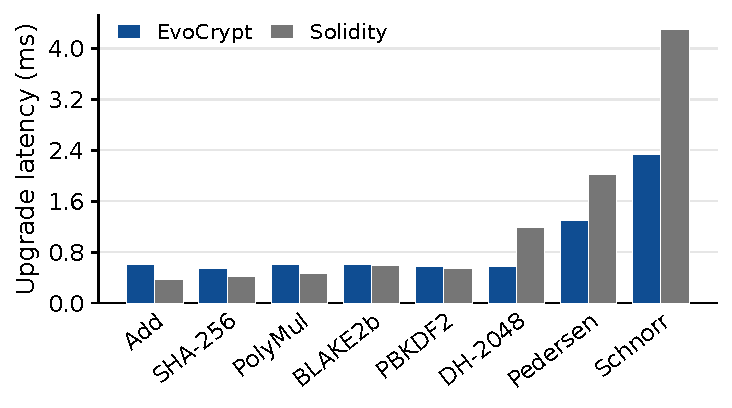
\includegraphics[width=\textwidth]{../image/figure_upgrade_latency_comparison.pdf}
\caption{Setup latency comparison between EvoCrypt upgrade and Solidity contract deployment.}
\label{fig:upgrade-latency}
\end{figure}

On lightweight algorithms, the two setup paths remained close in latency. For Add, SHA-256, BLAKE2b, and PBKDF2, mean upgrade latency stayed below 0.6~ms for EvoCrypt and below 0.6~ms for Solidity, with the largest gap on the non-cryptographic Add baseline (0.60~ms versus 0.37~ms). As algorithm complexity increased, EvoCrypt reduced setup latency relative to contract deployment. For DH-2048, PedersenCommit, and SchnorrVerify, EvoCrypt required 0.58--2.34~ms, whereas Solidity required 1.18--4.30~ms. The largest relative gain appeared on SchnorrVerify, where the upgrade path completed in 2.34~ms compared with 4.30~ms for contract deployment. These latency results report network-wide upgrade duration as defined in Section~\ref{sec5.1}: Geth-side handling through all evaluated nodes, excluding network propagation and consensus delay. They do not include upgrade-window availability for unrelated EVM traffic.

\subsection{Execution Efficiency}\label{sec5.3}

The execution-efficiency experiment evaluated steady-state invocation cost after each algorithm had been made callable. Figure~\ref{fig:execution-latency} compares mean \texttt{eth\_call} latency across EvoCrypt, Solidity, and Native algorithm paths, and Figure~\ref{fig:execution-gas} compares \texttt{gasEstimate} for EvoCrypt and Solidity. Each path was measured after warm-up calls using repeated \texttt{eth\_call} samples on the evaluated private-chain prototype.

\begin{figure}[!tb]
\centering
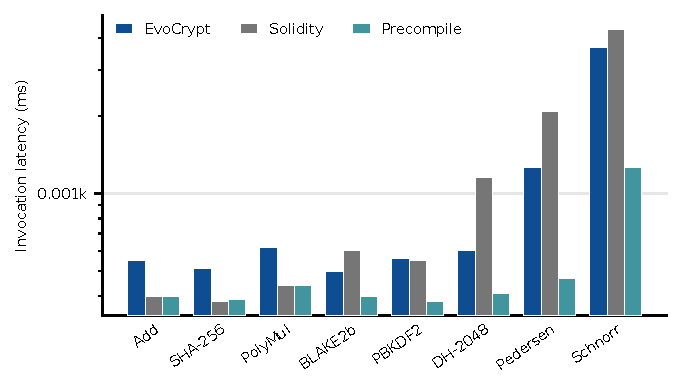
\includegraphics[width=\textwidth]{../image/figure_execution_latency_comparison.pdf}
\caption{Execution latency comparison among EvoCrypt, Solidity contract execution, and Native algorithm.}
\label{fig:execution-latency}
\end{figure}

\begin{figure}[!tb]
\centering
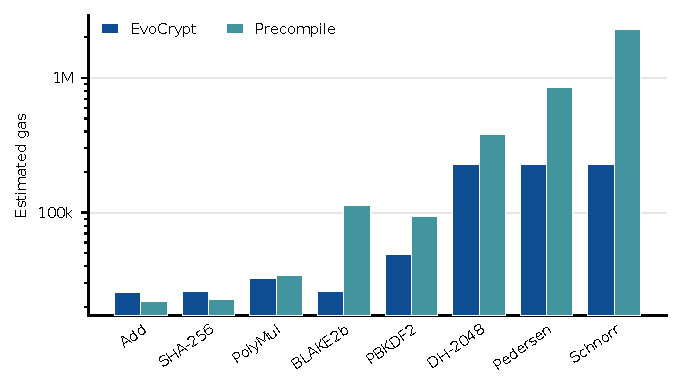
\includegraphics[width=\textwidth]{../image/figure_execution_gas_comparison.pdf}
\caption{Invocation \texttt{gasEstimate} comparison between EvoCrypt and Solidity contract execution.}
\label{fig:execution-gas}
\end{figure}

Native algorithm remained the fastest path on every algorithm, with mean latency between 0.38~ms (PBKDF2) and 1.26~ms (SchnorrVerify). EvoCrypt tracked Native algorithm closely on lightweight workloads: for Add, SHA-256, BLAKE2b, PBKDF2, and PolynomialMul, EvoCrypt latency remained within 0.50--0.62~ms, whereas Solidity stayed within 0.38--0.60~ms on the same set. On heavier cryptographic workloads, EvoCrypt reduced invocation latency relative to Solidity while remaining above Native algorithm. For DH-2048, PedersenCommit, and SchnorrVerify, EvoCrypt required 0.60, 1.26, and 3.67~ms, respectively, compared with 1.15, 2.07, and 4.33~ms through Solidity and 0.41, 0.47, and 1.26~ms through Native algorithm. SchnorrVerify therefore remained the clearest tail case: although EvoCrypt improved on Solidity, it still exceeded Native algorithm by roughly 2.9$\times$ on mean \texttt{eth\_call} latency.

The gas comparison makes the amplification effect directly visible. Solidity executions pay for the expanded EVM instruction sequence, so their estimates grew sharply with algorithmic complexity: Blake2bSum256, PedersenCommit, and SchnorrVerify required 113,059, 853,145, and 2,301,691 gas through contract execution. EvoCrypt instead charges the registered algorithm-level price, and its estimates for the same workloads were 25,801, 225,695, and 229,437 gas, up to an order of magnitude lower. For Add, SHA-256, and PolynomialMul, whose Solidity expansions remain short, the two contract-facing paths stayed within 13--15\% of each other, which is consistent with the amplification account: the separation between the two paths appears exactly where the instruction expansion grows. These numbers describe the current prototype invocation pricing model only; they are not receipt-level \texttt{gasUsed} measurements, and the registered prices are experimental parameters rather than a calibrated schedule. The comparison therefore demonstrates the decoupling mechanism and meters the Solidity side, rather than establishing a specific magnitude of gas savings.

\section{Conclusion}\label{sec6}

This paper presented an upgradable Cryptographic Coprocessor for the EVM. The central contribution is to separate a stable contract-facing invocation interface from client-side WASM module implementations, so that cryptographic algorithms can be managed as replaceable modules while ordinary EVM execution remains outside the upgrade mechanism. By routing calls through that interface instead of in-contract Solidity implementations, the design targets both the engineering difficulty and the opcode-level gas amplification that motivate the Solidity baselines evaluated in Section~\ref{sec5}, replacing per-instruction metering with the algorithm-level schedule~\eqref{eq:gas-price}. The upgrade protocol combines on-chain metadata~\eqref{eq:version-metadata}, off-chain asynchronous WASM preparation, and the height-based selector~\eqref{eq:version-select}.

The Geth prototype supports the design under the evaluated private-chain scenarios. The upgrade-efficiency experiment showed that publishing algorithms through the coprocessor upload path reduced network-wide upgrade duration---client-side Geth handling only, excluding network propagation and consensus---relative to redeploying equivalent Solidity implementations on several complex workloads, with SchnorrVerify as the clearest example. The execution-efficiency experiment showed that Native algorithm remained the fastest path, while EvoCrypt stayed within the millisecond range on lightweight algorithms and outperformed Solidity on DH-2048, PedersenCommit, and SchnorrVerify; SchnorrVerify nevertheless remained the clearest tail case relative to Native algorithm. Upgrade consistency remains a protocol property discussed through the Activation Block and forced-upgrade preparation policy rather than a separate experiment.

The current result has clear boundaries. It does not prove zero-downtime service availability, formal WASM sandbox security theorems, behavior when forced preparation cannot complete, state-root equality during upgrades, or consensus safety for arbitrary network sizes. Future work should calibrate the algorithm-level gas price schedule against measured execution cost, harden the upgrade channel against DoS and data-availability saturation attacks, define stricter ABI-version compatibility rules, validate additional cryptographic algorithms and WASM toolchains on further OS and architecture combinations, and design separate consistency and forced-preparation failure evaluations if those properties are later claimed experimentally.


\bibliographystyle{splncs04}
\bibliography{sn-bibliography}

\end{document}
